% TCC

\documentclass[
	12pt,					% tamanho da fonte
	%openright,				% capítulos começam em pág ímpar (insere página vazia caso preciso)
	oneside,				% twoside para impressão em recto e verso. Oposto a oneside
	a4paper,				% tamanho do papel. 
	chapter=TITLE,			% títulos de capítulos convertidos em letras maiúsculas
	%section=TITLE,			% títulos de seções convertidos em letras maiúsculas
	%subsection=TITLE,		% títulos de subseções convertidos em letras maiúsculas
	%subsubsection=TITLE,	% títulos de subsubseções convertidos em letras maiúsculas
	english,				% idioma adicional para hifenização
	brazil					% o último idioma é o principal do documento
	]{abntex2}


% Pacotes básicos 
\usepackage{times}				% Usa a fonte times roman			
\usepackage[T1]{fontenc}		% Selecao de codigos de fonte.
\usepackage[utf8]{inputenc}		% Codificacao do documento (conversão automática dos acentos)
\usepackage{indentfirst}		% Indenta o primeiro parágrafo de cada seção.
\usepackage{color}				% Controle das cores
\usepackage{graphicx}			% Inclusão de gráficos
\usepackage{microtype} 			% para melhorias de justificação
\usepackage{multirow}			% Para mesclar linhas
\usepackage{amsmath}			%¨Módulo matemático
\usepackage{csquotes}			% Aspas

% Pacotes de citações
\usepackage[brazilian,hyperpageref]{backref}	% Paginas com as citações na bibl
\usepackage[alf]{abntex2cite}					% Citações padrão ABNT



% Configurações do pacote backref
% Usado sem a opção hyperpageref de backref
\renewcommand{\backrefpagesname}{Citado na(s) página(s):~}
% Texto padrão antes do número das páginas
\renewcommand{\backref}{}
% Define os textos da citação
\renewcommand*{\backrefalt}[4]{
	\ifcase #1 %
		Nenhuma citação no texto.%
	\or
		Citado na página #2.%
	\else
		Citado #1 vezes nas páginas #2.%
	\fi}%


% Informações de dados para CAPA e FOLHA DE ROSTO
\titulo{Biblioteca de Tomada de Decisão com Lógica Paraconsistente para jogos de cartas}
\autor{
	Bruno de Paula Silva - C992534 \\
	Daniel Sousa David De Oliveira - D137GC0 \\
	Gustavo Felipe De Santana Marques - C993AH8 \\
	Marcelo Bueno Silva - N805CA0 \\
	Wesley Luiz Carvalho Silva - C993077}
\local{São Paulo}
\data{2019}
\orientador{Profª. Dr.a Amanda Luiza S. Pereira}
\instituicao{Universidade Paulista - UNIP}
\tipotrabalho{TCC}
\preambulo{Trabalho apresentado para aproveitamento da disciplina Trabalho de Curoso II , do curoso de Ciência da Computação, Da Universidade Paulista - UNIP Campus Cidade Universitária.}




% Configurações de aparência do PDF final
\definecolor{blue}{RGB}{0,0,0} % alterando o aspecto da cor azul

% informações do PDF
\makeatletter
\hypersetup{
     	%pagebackref=true,
		pdftitle={\@title}, 
		pdfauthor={\@author},
    	pdfsubject={\imprimirpreambulo},
	    pdfcreator={LaTeX with abnTeX2},
		pdfkeywords={abnt}{latex}{abntex}{abntex2}{trabalho acadêmico}, 
		colorlinks=true,       		% false: boxed links; true: colored links
    	linkcolor=blue,          	% color of internal links
    	citecolor=blue,        		% color of links to bibliography
    	filecolor=magenta,      	% color of file links
		urlcolor=blue,
		bookmarksdepth=4
}
\makeatother


% Posiciona figuras e tabelas no topo da página quando adicionadas sozinhas
% em um página em branco. Ver https://github.com/abntex/abntex2/issues/170
\makeatletter
\setlength{\@fptop}{5pt} % Set distance from top of page to first float
\makeatother



% Possibilita criação de Quadros e Lista de quadros.
% Ver https://github.com/abntex/abntex2/issues/176

\newcommand{\quadroname}{Quadro}
\newcommand{\listofquadrosname}{Lista de quadros}

\newfloat[chapter]{quadro}{loq}{\quadroname}
\newlistof{listofquadros}{loq}{\listofquadrosname}
\newlistentry{quadro}{loq}{0}

% configurações para atender às regras da ABNT
\setfloatadjustment{quadro}{\centering}
\counterwithout{quadro}{chapter}
\renewcommand{\cftquadroname}{\quadroname\space} 
\renewcommand*{\cftquadroaftersnum}{\hfill--\hfill}

\setfloatlocations{quadro}{hbtp} % Ver https://github.com/abntex/abntex2/issues/176

% Espaçamentos entre linhas e parágrafos 
\setlength{\parindent}{1.25cm} 	% O tamanho do parágrafo é dado por
\setlength{\parskip}{0.2cm} 	% Controle do espaçamento entre um parágrafo e outro


\makeindex 	% compila o indice


\begin{document} 		% Início do documento

\selectlanguage{brazil} % Seleciona o idioma do documento (conforme pacotes do babel)

\frenchspacing  		% Retira espaço extra obsoleto entre as frases.

% ----------------------------------------------------------
% ELEMENTOS PRÉ-TEXTUAIS
% ----------------------------------------------------------

\renewcommand{\imprimircapa}{
  \begin{capa}
    \center
    \ABNTEXchapterfont\Large Universidade Paulista - UNIP
    
    \vspace*{1cm}
    
    {\ABNTEXchapterfont\large\imprimirautor}

    \vfill
    \begin{center}
    \ABNTEXchapterfont\bfseries\LARGE\imprimirtitulo
    \end{center}
    \vfill
    
    \large\imprimirlocal

    \large\imprimirdata
    
    \vspace*{1cm}
  \end{capa}
}
\imprimircapa						% Inserir Capa

% folha de rosto 

\makeatletter

\renewcommand{\folhaderostocontent}{
\begin{center}
    
{\ABNTEXchapterfont\large\imprimirautor}

\vspace*{\fill}\vspace*{\fill}

\begin{center}
\ABNTEXchapterfont\bfseries\Large\imprimirtitulo
\end{center}

\vspace*{\fill}

\abntex@ifnotempty{\imprimirpreambulo}{
  	\hspace{.45\textwidth}
  	\begin{minipage}{.5\textwidth}
 	\SingleSpacing
 	\imprimirpreambulo
 	\end{minipage}
 	\vspace*{\fill}

	\hspace{.45\textwidth}
	Orientadora: \imprimirorientador
}

\vspace*{\fill}

{\large\imprimirlocal}

\par

{\large\imprimirdata}
\vspace*{1cm}
\end{center}
}
\imprimirfolhaderosto 

\makeatother

 				% Inserir Folha de rosto

% % Isto é um exemplo de Ficha Catalográfica, ou ``Dados internacionais de
% catalogação-na-publicação''. Você pode utilizar este modelo como referência. 
% Porém, provavelmente a biblioteca da sua universidade lhe fornecerá um PDF
% com a ficha catalográfica definitiva após a defesa do trabalho. Quando estiver
% com o documento, salve-o como PDF no diretório do seu projeto e substitua todo
% o conteúdo de implementação deste arquivo pelo comando abaixo:
%
% \begin{fichacatalografica}
%     \includepdf{fig_ficha_catalografica.pdf}
% \end{fichacatalografica}		% Inserir a ficha bibliografica

% % Inserir errata

\begin{errata}
Elemento opcional da \citeonline[4.2.1.2]{NBR14724:2011}. Exemplo:

\vspace{\onelineskip}

FERRIGNO, C. R. A. \textbf{Tratamento de neoplasias ósseas apendiculares com
reimplantação de enxerto ósseo autólogo autoclavado associado ao plasma
rico em plaquetas}: estudo crítico na cirurgia de preservação de membro em
cães. 2011. 128 f. Tese (Livre-Docência) - Faculdade de Medicina Veterinária e
Zootecnia, Universidade de São Paulo, São Paulo, 2011.

\begin{table}[htb]
\center
\footnotesize
\begin{tabular}{|p{1.4cm}|p{1cm}|p{3cm}|p{3cm}|}
  \hline
   \textbf{Folha} & \textbf{Linha}  & \textbf{Onde se lê}  & \textbf{Leia-se}  \\
    \hline
    1 & 10 & auto-conclavo & autoconclavo\\
   \hline
\end{tabular}
\end{table}

\end{errata} 					% Inserir errata

% % Isto é um exemplo de Folha de aprovação, elemento obrigatório da NBR
% 14724/2011 (seção 4.2.1.3). Você pode utilizar este modelo até a aprovação
% do trabalho. Após isso, substitua todo o conteúdo deste arquivo por uma
% imagem da página assinada pela banca com o comando abaixo:
%
% \begin{folhadeaprovacao}
% \includepdf{folhadeaprovacao_final.pdf}
% \end{folhadeaprovacao}
%
\begin{folhadeaprovacao}

  \begin{center}
    {\ABNTEXchapterfont\large\imprimirautor}

    \vspace*{\fill}\vspace*{\fill}
    \begin{center}
      \ABNTEXchapterfont\bfseries\Large\imprimirtitulo
    \end{center}
    \vspace*{\fill}
    
    \hspace{.45\textwidth}
    \begin{minipage}{.5\textwidth}
        \imprimirpreambulo
    \end{minipage}%
    \vspace*{\fill}
   \end{center}
        
   Trabalho aprovado. \imprimirlocal, 24 de novembro de 2012:

   \assinatura{\textbf{\imprimirorientador} \\ Orientador} 
   \assinatura{\textbf{Professor} \\ Convidado 1}
   \assinatura{\textbf{Professor} \\ Convidado 2}
   %\assinatura{\textbf{Professor} \\ Convidado 3}
   %\assinatura{\textbf{Professor} \\ Convidado 4}
      
   \begin{center}
    \vspace*{0.5cm}
    {\large\imprimirlocal}
    \par
    {\large\imprimirdata}
    \vspace*{1cm}
  \end{center}
  
\end{folhadeaprovacao} 		% Inserir folha de aprovação

% % ---
% Dedicatória
% ---
\begin{dedicatoria}
   \vspace*{\fill}
   \centering
   \noindent
   \textit{ Este trabalho é dedicado às crianças adultas que,\\
   quando pequenas, sonharam em se tornar cientistas.} \vspace*{\fill}
\end{dedicatoria}
% --- 			% Dedicatória

% % ---
% Agradecimentos
% ---
\begin{agradecimentos}
Os agradecimentos principais são direcionados à Gerald Weber, Miguel Frasson,
Leslie H. Watter, Bruno Parente Lima, Flávio de Vasconcellos Corrêa, Otavio Real
Salvador, Renato Machnievscz\footnote{Os nomes dos integrantes do primeiro
projeto abn\TeX\ foram extraídos de
\url{http://codigolivre.org.br/projects/abntex/}} e todos aqueles que
contribuíram para que a produção de trabalhos acadêmicos conforme
as normas ABNT com \LaTeX\ fosse possível.

Agradecimentos especiais são direcionados ao Centro de Pesquisa em Arquitetura
da Informação\footnote{\url{http://www.cpai.unb.br/}} da Universidade de
Brasília (CPAI), ao grupo de usuários
\emph{latex-br}\footnote{\url{http://groups.google.com/group/latex-br}} e aos
novos voluntários do grupo
\emph{\abnTeX}\footnote{\url{http://groups.google.com/group/abntex2} e
\url{http://www.abntex.net.br/}}~que contribuíram e que ainda
contribuirão para a evolução do \abnTeX.

\end{agradecimentos} 			% Agradecimentos

% % ---
% Epígrafe
% ---
\begin{epigrafe}
    \vspace*{\fill}
	\begin{flushright}
		\textit{``Não vos amoldeis às estruturas deste mundo, \\
		mas transformai-vos pela renovação da mente, \\
		a fim de distinguir qual é a vontade de Deus: \\
		o que é bom, o que Lhe é agradável, o que é perfeito.\\
		(Bíblia Sagrada, Romanos 12, 2)}
	\end{flushright}
\end{epigrafe} 				% Epígrafe

% % resumo em português
\setlength{\absparsep}{18pt} % ajusta o espaçamento dos parágrafos do resumo
\begin{resumo}
 Segundo a \citeonline[3.1-3.2]{NBR6028:2003}, o resumo deve ressaltar o
 objetivo, o método, os resultados e as conclusões do documento. A ordem e a extensão
 destes itens dependem do tipo de resumo (informativo ou indicativo) e do
 tratamento que cada item recebe no documento original. O resumo deve ser
 precedido da referência do documento, com exceção do resumo inserido no
 próprio documento. (\ldots) As palavras-chave devem figurar logo abaixo do
 resumo, antecedidas da expressão Palavras-chave:, separadas entre si por
 ponto e finalizadas também por ponto.

 \textbf{Palavras-chave}: latex. abntex. editoração de texto.
\end{resumo}

% resumo em inglês
\begin{resumo}[Abstract]
 \begin{otherlanguage*}{english}
   This is the english abstract.

   \vspace{\onelineskip}
 
   \noindent 
   \textbf{Keywords}: latex. abntex. text editoration.
 \end{otherlanguage*}
\end{resumo} 					% Resumo em português e inglês

% inserir lista de ilustrações
\pdfbookmark[0]{\listfigurename}{lof}
\listoffigures*
\cleardoublepage

% inserir lista de quadros
% \pdfbookmark[0]{\listofquadrosname}{loq}
% \listofquadros*
% \cleardoublepage

% inserir lista de tabelas
\pdfbookmark[0]{\listtablename}{lot}
\listoftables*
\cleardoublepage

% inserir lista de abreviaturas e siglas
% \begin{siglas}
%   \item[ABNT] Associação Brasileira de Normas Técnicas
%   \item[abnTeX] ABsurdas Normas para TeX
% \end{siglas}

% inserir lista de símbolos
% \begin{simbolos}
%   \item[$ \Gamma $] Letra grega Gama
%   \item[$ \Lambda $] Lambda
%   \item[$ \zeta $] Letra grega minúscula zeta
%   \item[$ \in $] Pertence
% \end{simbolos} 					% Inseir listas

% inserir o sumario
\pdfbookmark[0]{\contentsname}{toc}
\tableofcontents*
\cleardoublepage
								% inseir sumário


% ----------------------------------------------------------
% ELEMENTOS TEXTUAIS
% ----------------------------------------------------------
\textual

%Introdução

\chapter{Introdução}

Este trabalho acadêmico demonstra a aplicação da Lógica Paraconsistente Anotada (LPA), em jogos do gênero \textit{Tranding Card Games} (Jogos de Cartas Colecionáveis – TCG), através da criação de uma biblioteca de \dfrac{Tomada}{den} de Decisão que implementa a Lógica Paraconsistente Anotada Evidencial (LPA E$\tau$), além disso será criado um jogo de cartas que utiliza a biblioteca para demonstrar as suas funcionalidades.

Com parte do senso comum, as pessoas acreditam que os jogos têm como única finalidade entreter ignorando as diversas opções que um jogo eletrônico pode trazer para auxiliar o desenvolvimento humano, de modo que a utilização dos jogos de forma educacional ou para resolver problemas usando raciocínio lógico pode trazer benefícios à saúde \cite{fabio-luis-lpa}.

A LPA é uma lógica não clássica que admite contradições e incertezas, é uma boa solução para fazer tratamento de situações reais, no qual a Lógica Clássica, por ser binária, se mostra ineficaz ou impossibilitada de ser aplicada \cite{metodos-lpa-2006}. Assim possibilita as mais variadas aplicações em áreas tais como computação, robótica, tráfego aéreo e de trens, distribuição de energia em grandes usinas, programação, redes neurais, pesquisa operacional entre outras \cite{tomda-decisao-lpa-2011}.

Uma biblioteca é uma coleção de subprogramas ou um programa que facilita o desenvolvimento de sistemas, no núcleo da biblioteca desenvolvida será utilizado a
LPA. Dessa forma a biblioteca implementada no jogo será responsável por tomar as decisões dos resultados de batalha, sendo o intuito de criar um software que pode ser reutilizável por outros, iniciando um estudo da aplicação da LPA em jogos TGC.

Será explicado como a biblioteca foi desenvolvida e implementada no jogo, juntamente com a sua documentação para utilização. Também será relatado como o
jogo foi desenvolvido, quais ferramentas e metodologias foram utilizadas e quais resultados que foram obtidos em vantagem com a utilização da LPA.

Este documento está estruturado nos seguintes tópicos, \textit{1 - Introdução} apresenta o projeto, os objetivos e as justificativas. No capítulo \textit{2 - Referência Teórica} é
exposta a base conceitual do projeto. Na seção seguinte \textit{3 - Materiais e Métodos} é retratada a metodologia utilizada para desenvolvimento da prototipagem além das ferramentas utilizadas no processo. [EM CONSTRUÇÃO]

Terminada a descrição da estrutura do trabalho, prossegue para \textit{capítulo 2 - Referência Teórica}.

\section{Justificativa}

No desenvolvimento de jogos de cartas, é encontrado diversas bibliotecas disponibilizado na \textit{Unity Asset Store}, com uso de lógica clássica, que uma proposição é classificada como verdadeira ou falsa. Não há qualquer outra possível alternativa, ou algo é Verdadeiro ou exclusivamente Falso \cite{aspectos-lpa-2013}.

A lógica paraconsistente introduz duas novas categorias além do Verdadeiro e do Falso. Podemos ter proposições classificadas como Verdadeiras, Falsas, Inconsistentes ou Paracompletas. Para uma proposição ser classificada com Inconsistente tem haver uma evidência sugere que ela seja Verdadeira e outra evidência sugere que ela é Falsa, Agora quando não tem evidência Verdadeira nem tampouco que ela seja Falsa a proposição é classificada como Paracompleta \cite{aspectos-lpa-2013}.

Sendo que a Logica Paraconsistente é utilizado em outras áreas e não é utilizado especificamente em jogos e cartas. Portanto a proposta do projeto é desenvolver uma biblioteca aplicando Tomada de Decisão com Lógica Paraconsistente ao invés do Logica clássica, para auxiliar no processo decisório de uma forma ágil e eficiente.


\section{Validação Empírica}

A LPA é uma lógica não clássica que aceita contradições. A partir disso criar um cenário de jogo de cartas para demonstrar o uso da
paraconsistente. Para exemplificar, foram criadas quatro cartas com atributos de força e velocidade com valores favoráveis e desfavoráveis de acordo com arma e idade conforme a tabela \ref{tab:cartas}.

\begin{table}[htb]
	\centering
	\caption{Visualização das Cartas}
	\label{tab:cartas}
	\begin{tabular}{|l|l|l|l|l|l|}
		\hline
		\textbf{Carta}              & \textbf{Atributos}  & \textbf{Favorável} & \textbf{Desfavorável} & \textbf{Detalhes} & \textbf{Valor} \\ \hline
		\multirow{2}{*}{Arqueiro}   & \textit{Força}      & 20                 & 10                    & \textit{Arma}     & Arco e Flecha  \\ \cline{2-6} 
		& \textit{Velocidade} & 70                 & 35                    & \textit{Idade}    & 25             \\ \hline
		\multirow{2}{*}{Espadachim} & \textit{Força}      & 55                 & 20                    & \textit{Arma}     & Espada         \\ \cline{2-6} 
		& \textit{Velocidade} & 40                 & 20                    & \textit{Idade}    & 19             \\ \hline
		\multirow{2}{*}{Lanceiro}   & \textit{Força}      & 50                 & 10                    & \textit{Arma}     & Lança          \\ \cline{2-6} 
		& \textit{Velocidade} & 68                 & 35                    & \textit{Idade}    & 30             \\ \hline
		\multirow{2}{*}{Bárbaro}    & \textit{Força}      & 70                 & 50                    & \textit{Arma}     & Martelo        \\ \cline{2-6} 
		& \textit{Velocidade} & 60                 & 80                    & \textit{Idade}    & 40             \\ \hline
	\end{tabular}
	\fonte{Produzido pelos autores.}
\end{table}

O primeiro passo é realizar o processo de maximização, a partir do qual se obtém os maiores valores das evidências favoráveis e os menores das evidências
desfavoráveis, entre as cartas \textit{Arqueiro} e \textit{Espadachim}, repetindo o processo em relação às cartas \textit{Lanceiro} e \textit{Bárbaro}. Na sequência, realiza-se o processo de minimização, o qual consiste na obtenção dos menores valores das evidências favoráveis e dos maiores valores das evidências desfavoráveis, as quais foram maximizadas anteriormente.
Após realizar o processos de maximização e minimização nos dois atributos das cartas, obteve-se os seguintes valores:

\begin{figure}[htb]
	\caption{
		\label{fig:forca} 
		Valores
	}
	\begin{center}
		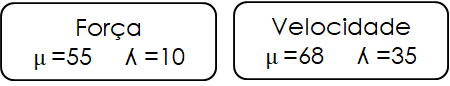
\includegraphics[scale=0.5]{imagens/valores.png}
	\end{center}
	\legend{Fonte: Produzido pelos autores.}

\end{figure}

Após a realização da maximização entre esses valores chegou-se ao seguinte resultado:

\begin{figure}[htb]
	\caption{
		\label{flg:max}
		Maximização
	}
	\begin{center}
		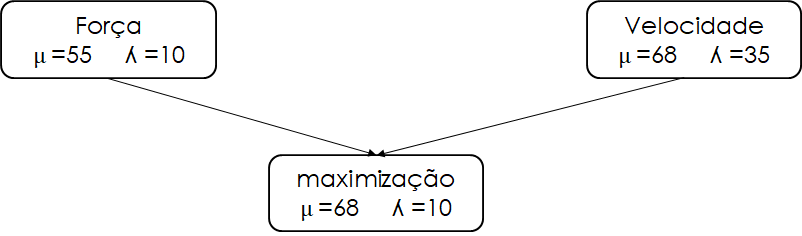
\includegraphics[scale=0.5]{imagens/max.png}
	\end{center}
	\legend{Fonte: Produzido pelos autores.}	
\end{figure}

Aplicando o grau de certeza e incerteza sobre esses valores a saída foi o seguinte estado lógico:

\begin{equation*}
	\begin{array}{cc}
	Gi = 0.68 + 0.1 -1 = -0.22 \\
	Gc = 0.68 - 0.1 = 0.58
	\end{array}
\end{equation*}

Através do estado lógico foi produzido o parecer analítico com uma tabela pré definida cujo resultado refere-se a porcentagem que as 4 cartas conseguem tirar de vida do adversário.

\newpage

\begin{table}[htb]
	\centering
	\caption{Relação entre o status e parecer analítico}
	\label{tab:analitica}
	\begin{tabular}{cc}
		\hline
		\multicolumn{1}{|c|}{\textbf{Status}} 	& \multicolumn{1}{c|}{\textbf{Parecer Analítico}} \\ \hline
		$V$               						& 100\%                      \\
		$F$               						& 0\%                        \\
		$T$               						& 0\%                        \\
		$\bot$									& 0\%                        \\
		$T \rightarrow V$             			& 20\%                       \\
		$T \rightarrow F$            			& 10\%                       \\
		$V \rightarrow \bot$            		& 16\%                       \\
		$F \rightarrow \bot$            		& 8\%                        \\
		$Qv \rightarrow T$            			& 50\%                       \\
		$Qv \rightarrow \bot$           		& 40\%                       \\
		$Qf \rightarrow T$            			& 6\%                        \\
		$Qf \rightarrow \bot$           		& 2\%                       
	\end{tabular}
	\fonte{Produzido pelos autores.}
\end{table}

O status obtido na maximização foi $T \rightarrow F$, conforme a tabela \ref{tab:analitica} a porcentagem seria de 10\%, com essa validação possuí a lógica que será aplicada para Tomada de Decisão no jogo, assim iniciar a criação da dinâmica do jogo.

\section{Objetivos}

O objetivo geral é desenvolver uma biblioteca de Tomada de Decisão que utilize a LPA com foco em jogos TCG com objetivo de, protótipo final, isso é, biblioteca com manual de utilização e jogo de demostração, com o intuito de ser utilizada por outros desenvolvedores de jogos de cartas


\section{Objetivos Específicos}
	\begin{itemize}
		\item Criar o modelo de paraconsistente a ser utilizado.
		\item Criar a biblioteca aplicando a LPA E$\tau$.
		\item Criar uma versão da biblioteca com valores fixo para uma implementação no jogo sem muitos problemas.
		\item Desenvolver uma segunda versão da biblioteca, permitindo que ela seja genérica o suficiente para atender diferentes regras de negócio em jogos TCG.
		\item Desenvolvimento da biblioteca.
		\item Construir um manual de utilização e documentação da biblioteca.
		\item Criar um jogo do gênero TCG que demonstre as funcionalidades da biblioteca.
		\item Gerar \textit{Asset} e disponibilizar na plataforma \textit{Unity Asset Store}.
		\item Criar a presente documentação descrevendo os materiais, métodos e referências utilizadas para a construção do projeto.
	\end{itemize}




%Referencial Teórico

\chapter{Referência Teórica}

Neste capitulo será descrito quais as referências que incentivaram a escolha do tema em questão.

\section{Lógica Paraconsistente}

A LPA teve como precursores o lógico russo N. A. Vasiliev e o lógico polonês J.Lukasiewicz. Os dois em 1910, publicaram trabalhos independentes, porém se restringiam a lógica aristotélica tradicional. Entre 1948 e 1954 o lógico polonês S.Jaskowski e o lógico brasileiro Newton C.A. da Costa, independentes construíram a LPA \cite[p. 27]{tomda-decisao-lpa-2011}.

Segundo \citeonline{introd-lpa-2010} dentre as várias ideias no âmbito das Lógicas não-Clássicas criou-se uma família de lógicas que teve como fundamento principal a  revogação do princípio da Não Contradição, a qual foi nomeada de Lógica Paraconsistente. Portanto, a LPA é uma Lógica não-Clássica que
revoga o princípio da Não Contradição e admite o tratamento de informações
contraditórias na sua estrutura teórica.

\section{Teoria dos jogos}

\section{Biblioteca}

\section{Engenharia de Software}

Visando melhorar a qualidade dos produtos de software e aumentar a produtividade no processo de desenvolvimento, surgiu a Engenharia de Software. A Engenharia de Software trata de aspectos relacionados ao estabelecimento de processos, métodos, técnicas, ferramentas e ambientes de suporte ao desenvolvimento de software \cite[p. 2]{eng-2014}.

\subsection{Metodologia}

\subsection{UML}

Particularmente no tocante à engenharia de software, a \textit{Unified Modeling Language} (Linguagem de Modelagem Unificada - UML) pode ser utilizada para modelar todas as etapas do processo de desenvolvimento de software, bem como produzir todos os artefatos de Software necessários à documentação dessas etapas \cite[p. 12]{eng-2015}.

Segundo o mesmo autor (\citeyear{eng-2015}), a linguagem UML, por meio de seus diagramas, permite a definição e design de \textit{threads} (tarefas) e processos, que permitem o desenvolvimento de sistemas distribuídos ou de programação concorrente. Da mesma maneira, permite a utilização dos chamados \textit{patterns} são, a grosso modo, soluções de programação utilizadas devido ao seu bom desempenho e a descrição de colaborações esquemas de interação entre objetos que resultam em um comportamento do sistema.

\subsection{RUP}

% Materiais e Métodos

\chapter{Materiais e Métodos}

Para a elaboração do presente trabalho foram adotadas técnicas e metodologias que serão mostrados nos próximos tópicos.

\section{Linguagem C\#}

C\# ou \textit{C Sharp} é uma linguagem de programação orientada a objetos desenvolvido pela Microsoft, que faz parte de sua plataforma .Net. Que foi baseado em C++ e/ou java.

\section{Plataforma Unity}

A plataforma Unity é conhecido como uma das melhores plataforma de desenvolvimento de jogos do mundo, justamente porque ela é potencializada em serviços e ferramentas sendo elas 2D e 3D.
Segundo \citeonline{unity-2019} \enquote{atualmente a plataforma domina 45\% do mercado global de desenvolvimentos de games, segundo a própria empresa; 34\% dos 1.000 maiores jogos mobile disponibilizado gratuitamente são feitos com a própria Unity.}

\section{Visual Studio}



\phantompart

% ----------------------------------------------------------
% ELEMENTOS PÓS-TEXTUAIS
% ----------------------------------------------------------
\postextual



\bibliography{references} % Referências bibliográficas

% Inicia os apêndices
% \begin{apendicesenv}

% \partapendices % Imprime uma página indicando o início dos apêndices

% \chapter{rup}

% \chapter{documentação Biblioteca}

% \end{apendicesenv}


% INDICE REMISSIVO
\phantompart
\printindex

\end{document}
